\documentclass[titlepage,11pt,twoside]{article}
\usepackage[dvips]{graphicx}

\usepackage{color}
\usepackage{mathtools}
\usepackage{amssymb}
\usepackage{hyperref}
\usepackage{natbib}
\usepackage{multirow}
%\usepackage{colortbl}
\usepackage[table]{xcolor}
\definecolor{lightgray}{gray}{0.9}
\usepackage[T1]{fontenc}

\usepackage{caption,setspace}
\captionsetup{font={footnotesize,stretch=1.5}}
\renewcommand{\baselinestretch}{1.2} 

\usepackage{tikz}
\usetikzlibrary{arrows}
\usetikzlibrary{shapes, positioning, calc} 


\newcommand{\bfU}{\mbox{\boldmath$\mathsf{U}$}}
\newcommand{\bfu}{\mbox{\boldmath$\mathsf{u}$}}
\newcommand{\hl}[1]{\textcolor{magenta}{#1}}
\newcommand{\RR}{\mathbb{R}}
\DeclareMathOperator*{\V}{V}
\DeclareMathOperator*{\argmax}{argmax}
\newcommand{\R}[1]{\texttt{#1}}
\newcommand{\acos}{\text{arccos}}

%\usepackage{helvet}
%\renewcommand{\familydefault}{\sfdefault}
%\renewcommand{\rmdefault}{\sfdefault} % Aria

\usepackage{arev}

%\begin{figure}[h]
%\centerline{\includegraphics{figure03.eps}}
%\caption{Projection of item discrimination vectors onto $V_{\theta_T}$ hyperplance for a six item three-dimensional approximate sample structure.}
%\end{figure}

%\raggedbottom
\flushbottom


%\firstpage{1}
%\setcounter{lastpage}{999}
\setcounter{secnumdepth}{3}


\begin{document}

Dear Editor,

\medskip

Please consider the attached research paper \emph{``Exploratory data structure comparisons: Three new visual tools based on Principal Component Analysis''} for publication in PLoS One.


\bigskip

Yours Sincerely,

\bigskip\bigskip

Anne Helby Petersen

Scientific Assistant

Section of Biostatistics

Faculty of Health and Medical Sciences

University of Copenhagen


\begin{itemize}
\item Summarize the study’s contribution to the scientific literature
\item Relate the study to previously published work
\item[Done] Specify the type of article (for example, research article, systematic review, meta-analysis, clinical trial)
\item[Not relevant] Describe any prior interactions with PLOS regarding the submitted manuscript
\item Suggest appropriate Academic Editors to handle your manuscript (see the full list of Academic Editors)
\item[Not relevant] List any opposed reviewers
\end{itemize}
\end{document}

%%%%%%%%%%%%%%%%%%%

% Hvad var meningen med nedenstående diagrammer? 
% De skal nok bare fjernes.

\begin{document}
\center
Model 1: \medskip \\
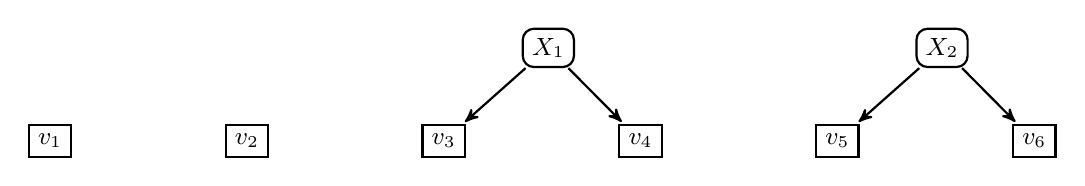
\begin{tikzpicture}[->,>=stealth',shorten >=1pt,auto, node distance=2.5cm,
  thick,main node/.style={rectangle, rounded corners,draw,font=\sffamily\small\normalfont},
  sq node/.style={rectangle,draw,font=\sffamily\small\normalfont}]
  \node[sq node] (1) {$v_1$};
  \node[sq node, right of = 1] (2) {$v_2$};
  \node[sq node, right of = 2] (3) {$v_3$};
  \node[sq node, right of = 3] (4) {$v_4$};
  \node[sq node, right of = 4] (5) {$v_5$};
  \node[sq node, right of = 5] (6) {$v_6$};
  \node[main node, above right=1cm of 3] (7) {$X_1$};
  \node[main node, above right=1cm of 5] (8) {$X_2$};
  \path[every node/.style={font=\sffamily\small}]
    (7) edge node  {} (3)
    (7) edge node {} (4)
    (8) edge node {} (5)
    (8) edge node {} (6);
 \end{tikzpicture}
\\
\bigskip
Model 2: \medskip \\
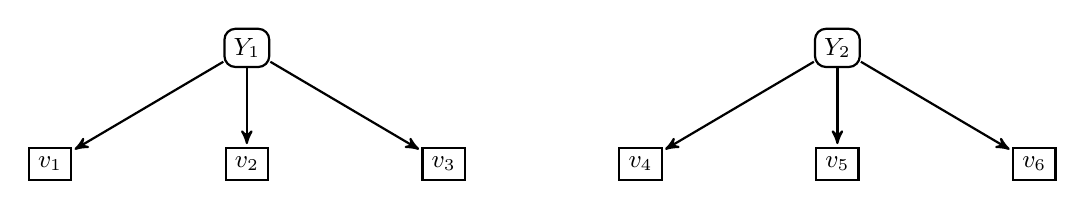
\begin{tikzpicture}[->,>=stealth',shorten >=1pt,auto, node distance=2.5cm,
  thick,main node/.style={rectangle, rounded corners,draw,font=\sffamily\small\normalfont},
  sq node/.style={rectangle,draw,font=\sffamily\small\normalfont}]
  \node[sq node] (1) {$v_1$};
  \node[sq node, right of = 1] (2) {$v_2$};
  \node[sq node, right of = 2] (3) {$v_3$};
  \node[sq node, right of = 3] (4) {$v_4$};
  \node[sq node, right of = 4] (5) {$v_5$};
  \node[sq node, right of = 5] (6) {$v_6$};
  \node[main node, above=1cm of 2] (7) {$Y_1$};
  \node[main node, above=1cm of 5] (8) {$Y_2$};
  \path[every node/.style={font=\sffamily\small}]
    (7) edge node  {} (1)
    (7) edge node {} (2)
    (7) edge node {} (3)
    (8) edge node {} (4)
    (8) edge node {} (5)
    (8) edge node {} (6);
 \end{tikzpicture}

\end{document}
